\documentclass{article}

\usepackage[a4paper, total={6in, 8in}]{geometry}
\usepackage{setspace}
\usepackage{lineno}
\usepackage{graphicx}

\title{Understanding the effects of date rounding in phylodynamics}
\author{Leo A. Featherstone$^{\ast,1}$, [Order TBA], Sebastian Duchene$^{\dagger,1}$}

\begin{document}

\maketitle
\linenumbers
$^{1}$ Peter Doherty Institute for Infection and Immunity, University of Melbourne, Australia.\\
*email: leo.featherstone@unimelb.edu.au

\section*{Abstract}
\textbf{Serving as a guideline for the message of the paper for now.}
Phylodynamic and genomic epidemiology frequently rely on the sampling times from pathogen isolates to make inference about the development of disease outbreaks over time. By calibrating a rate of substitution against epidemiological timescales, sampling times, in combination with genome sequence, allow for inferences such as the time of onset of an outbreak and intensity of transmission. However, for patient confidentiality, the exact sampling times for many sequences are not given, or rounded to a less precise amount of time such as month or year. Here, we show for the first time how and when such 'date-rounding' induces bias in epidemiological estimates. Broadly, this bias is often substantial, increases with the degree of rounding in provided sampling dates, and affect inference of all parameters including of time of onset and reproductive number. Finally, we close by proposing a solution that prioritises both patient confidentiality and accuracy of inference in genomic epidemiology, by proposing a basic form of encryption of dates in absolute time by translating them by an unknown number.

\begin{spacing}{1.5}
\section*{Introduction}
\begin{itemize}
    \item How and why rounding of dates occurs
    \item Types of rounding and presumed problems, including distorting clock signal (e.g. `stress' in the rtt?)
    \item Consider a figure to show the distortion in the phylogram and in an rtt?
    \item `effective number of mutations' do we still need this concept?
    \item That it might matter for the clock and what downstream parameters
\end{itemize}

Increased sharing of pathogen genome sequences has been a feature of responses to recent infectious disease threats. This is also the culmination of a broader trend that has build with advances in WGS. 

\section*{Results}
\subsection*{Results Overview}
\textbf{Points to hit}
\begin{itemize}
    \item Bias in all parameters
    \item $R_e$ / $R_0$ is biased upwards
    \item origin ispushed deeper in time, implicating a more severe longstanding outbreak
    \item Clock rate is increased, suggesting a faster rate of mutation
    \item This trend is worst for smaller datasets, where the duration of infection is shorter relative to the error induced in rounding
    \item By contrast TB is affected less, but we need the specificity for emergent outbreaks most
    \item Show that severity seems to correlate with relationship between error and timing, if I can motivate one in introduction
\end{itemize}

\subsection*{Simulation Study}

\begin{figure}[h]
\centering
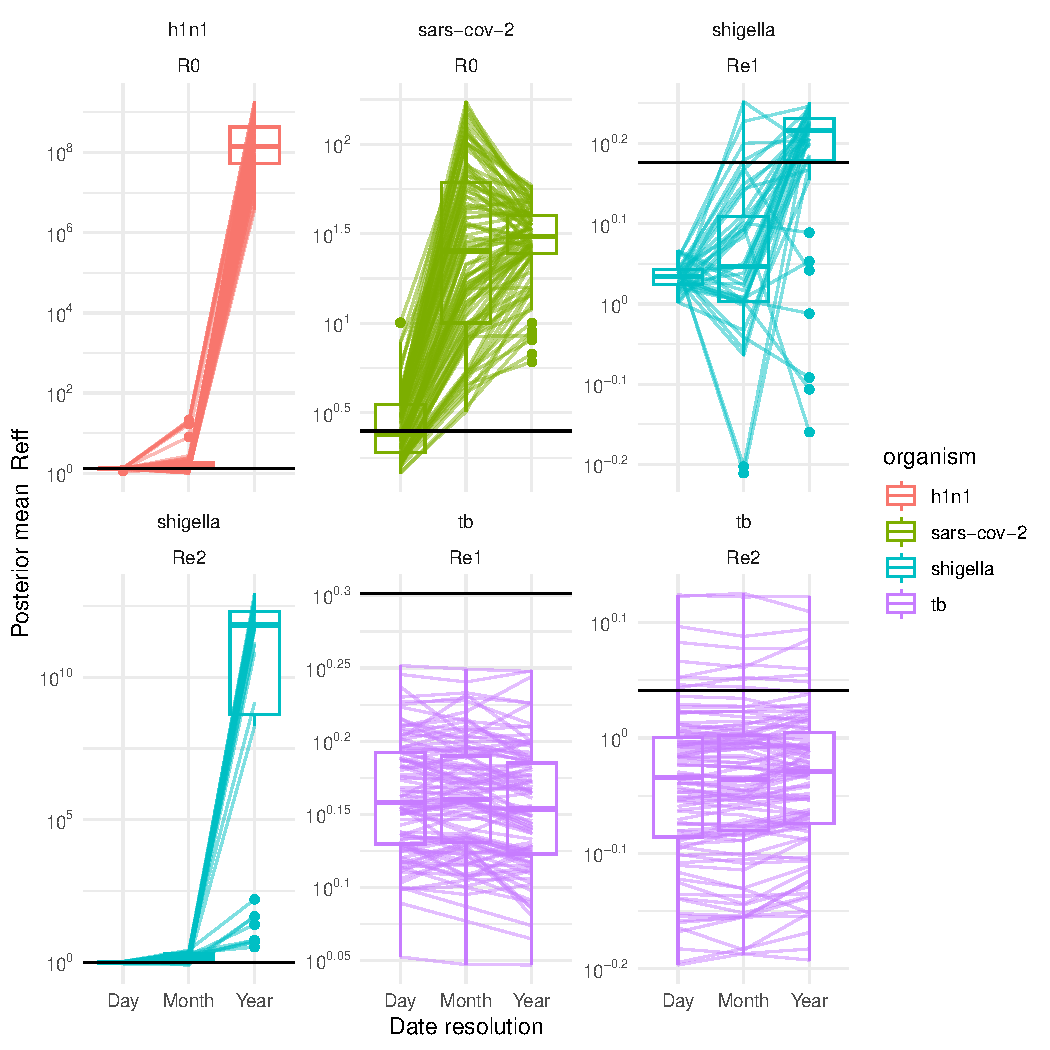
\includegraphics[width = 1\linewidth]{sim_Re_trajectory}
\caption{Mean posterior $R_0$ or $R_e$ for simulated datasets across each level of date resultion, separated over simulation conditions emulating each pathogen (n=100). I.e. One line connects mean posterior estimates for a single simulated datasets analyses under each data resultuiton codition. For H1N1 and SARS-CoV-2 conditions, reducing date resolution (left to right) corresponds to upwards bias mean posterior $R_0$ and $R_e$. For year, having idnetical dates corresponds to complete model mispecification and wholly implausible mean posterior $R_{\bullet}$ values. }
\label{simRe}
\end{figure}


\begin{figure}[h]
\centering
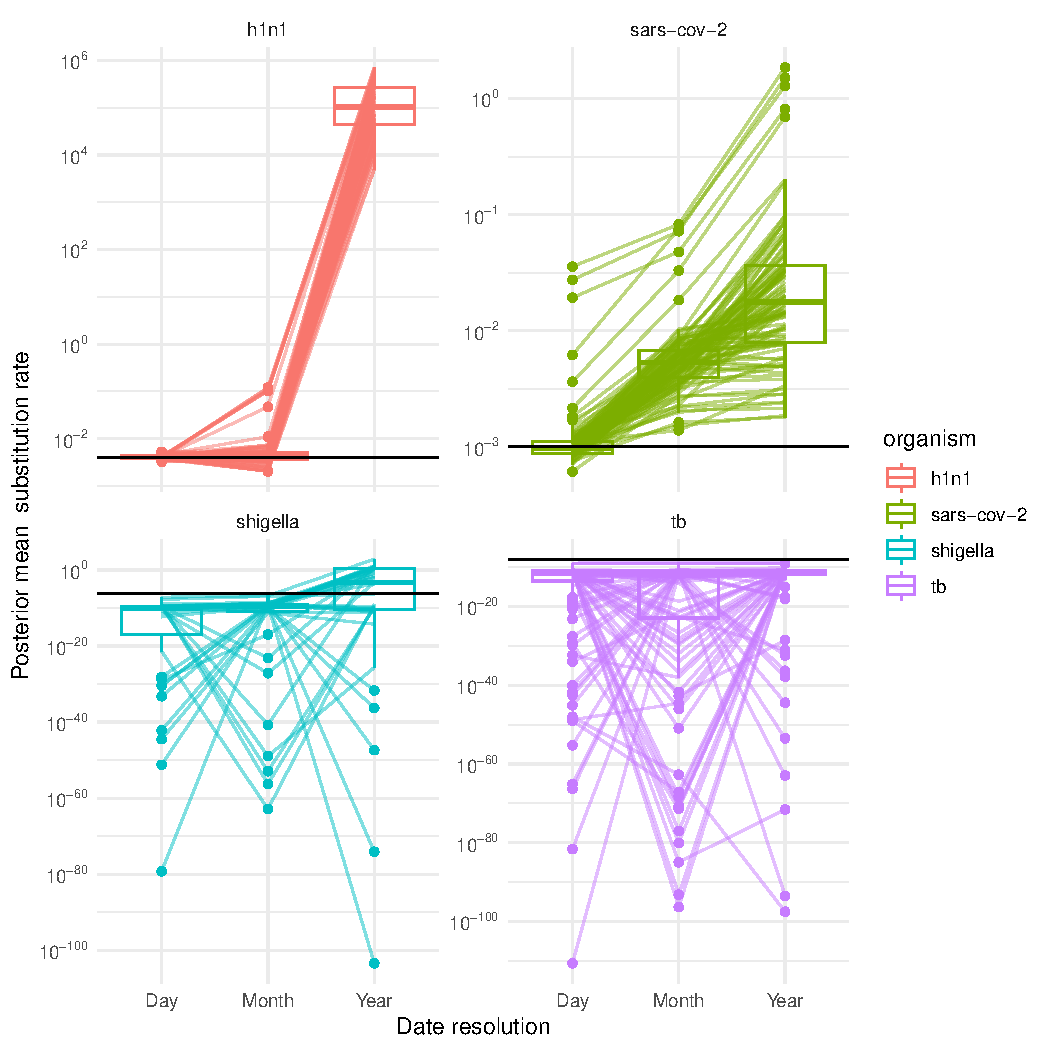
\includegraphics[width = 1\linewidth]{sim_clock_trajectory}
\caption{Mean posterior evolutionary rate for simulated datasets across each level of date resultion, separated over simulation conditions emulating each pathogen (n=100). I.e. One line connects mean posterior estimates for a single simulated datasets analyses under each data resultuiton codition. For H1N1 and SARS-CoV-2 conditions, reducing date resolution (left to right) corresponds to upwards bias mean posterior evolutionary rate. For Shigella this effect still present, wlthough diminshed, and estimates for TB appear relatively stable.}
\label{simClock}
\end{figure}

\begin{figure}[h]
\centering
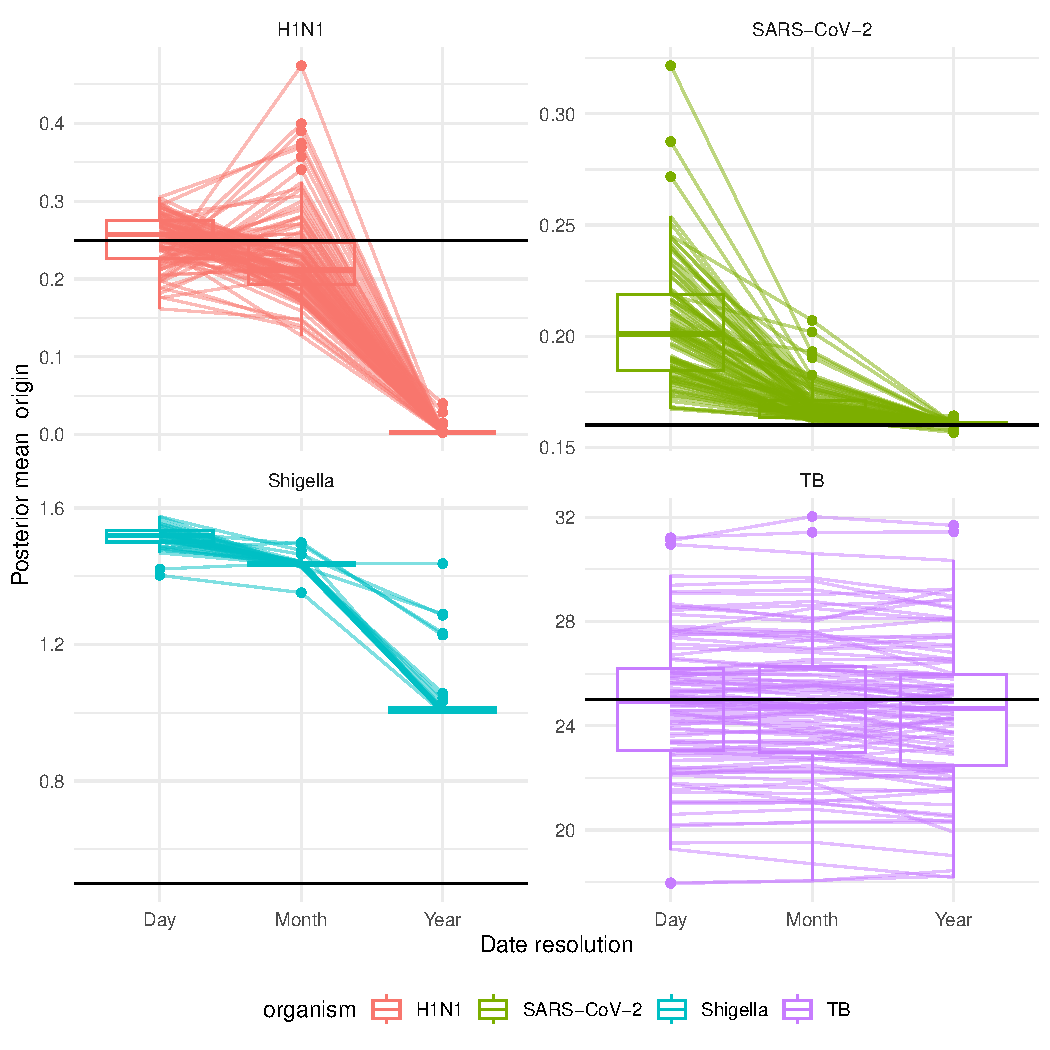
\includegraphics[width = 1\linewidth]{sim_origin_trajectory}
\caption{Mean posterior origin for simulated datasets across each level of date resultion, separated over simulation conditions emulating each pathogen (n=100). I.e. One line connects mean posterior estimates for a single simulated datasets analyses under each data resultuiton codition. TO FINISh}
\label{simOrigin}
\end{figure}


\subsection*{Empirical Results}
\begin{itemize}
	\item Here, do I want to group viruses or do each individually? Depends how much I say in the general results overview part.
\end{itemize}


\begin{table}[ht]
\centering
\begin{tabular}{rllrlrlrlrlrlrl}
  \hline
 & organism & resolution & meanR0 & R0HPD & meanRe1 & Re1HPD & meanRe2 & Re2HPD & meanP & pHPD & meanDelta & deltaHPD & meanOrigin & originHPD \\ 
  \hline
1 & h1n1 & Day & 1.08 & [1.05169500944395, 1.11375862585647] &  & [NA, NA] &  & [NA, NA] & 0.01 & [0.00659569715253315, 0.0155842605488171] &  & [NA, NA] & 0.42 & [0.345213671924637, 0.558121100896718] \\ 
  2 & h1n1 & Month & 1.14 & [1.11518272001637, 1.17471931965058] &  & [NA, NA] &  & [NA, NA] & 0.01 & [0.00361938676257238, 0.0104026209789307] &  & [NA, NA] & 0.42 & [0.337879801550098, 0.557463461023221] \\ 
  3 & h1n1 & Year & 115948630.02 & [89603766.8312088, 145241108.540186] &  & [NA, NA] &  & [NA, NA] & 0.26 & [0.00197330058636351, 0.937884688648121] &  & [NA, NA] & 0.00 & [2.38970001694422e-09, 3.69219852642698e-09] \\ 
  4 & sars-cov-2 & Day & 1.20 & [0.918485254309922, 1.57665249346316] &  & [NA, NA] &  & [NA, NA] &  & [NA, NA] & 81.93 & [51.3470583146435, 122.508381210983] & 0.15 & [0.143051162148834, 0.163538179019229] \\ 
  5 & sars-cov-2 & Month & 5.95 & [3.83426191124472, 9.17572009709929] &  & [NA, NA] &  & [NA, NA] &  & [NA, NA] & 98.36 & [62.3512625646851, 142.745878617093] & 0.17 & [0.169653799613119, 0.175910154585298] \\ 
  6 & sars-cov-2 & Year & 18.54 & [10.3581474274774, 29.3223275555288] &  & [NA, NA] &  & [NA, NA] &  & [NA, NA] & 44.24 & [26.2174407698453, 72.1746563934306] & 0.14 & [0.142042804540097, 0.146467722540314] \\ 
  7 & shigella & Day &  & [NA, NA] & 1.08 & [1.05676572410561, 1.11583512872131] & 0.98 & [0.973198366643138, 0.992273637904491] & 0.00 & [0.0004325857159814, 0.00112345940490641] &  & [NA, NA] & 3.52 & [3.36151270018212, 3.67904354020509] \\ 
  8 & shigella & Month &  & [NA, NA] & 1.09 & [1.05727663310813, 1.12069886831528] & 0.98 & [0.973032652127982, 0.992413924409982] & 0.00 & [0.000437238641408346, 0.0011253065396057] &  & [NA, NA] & 3.51 & [3.33731168230983, 3.67479085529529] \\ 
  9 & shigella & Year &  & [NA, NA] & 1.15 & [1.11656965664599, 1.19787075434164] & 0.96 & [0.944971106656953, 0.968495167865325] & 0.00 & [0.000465835029962845, 0.00120357381987583] &  & [NA, NA] & 4.00 & [3.99573546496778, 4.0240794648419] \\ 
  10 & tb & Day &  & [NA, NA] & 2.51 & [0.683584249035168, 4.8837661824016] & 1.30 & [0.697363295459474, 2.41372137032041] & 0.09 & [0.042641548799869, 0.149249396475237] & 0.29 & [0.10405678454571, 0.602624728546814] & 23.09 & [16.3311964670633, 49.3144990334623] \\ 
  11 & tb & Month &  & [NA, NA] & 2.80 & [0.611546919439069, 5.13887513665705] & 1.39 & [0.732063056194756, 2.55383926975437] & 0.09 & [0.0414798888248787, 0.149180650208098] & 0.23 & [0.0997614587741593, 0.415771137190394] & 24.40 & [17.8598975325763, 50.6092849103327] \\ 
  12 & tb & Year &  & [NA, NA] & 2.76 & [0.493224025193359, 5.26000442897983] & 1.48 & [0.767673831981051, 2.84272295289379] & 0.09 & [0.0402890351928377, 0.146465920750652] & 0.22 & [0.0937158489385196, 0.398204703001644] & 25.62 & [18.0291125919234, 55.3423889520615] \\ 
   \hline
\end{tabular}
\end{table}

% latex table generated in R 4.3.0 by xtable 1.8-4 package
% Wed May 17 12:34:59 2023
\begin{table}[ht]
\centering
\begin{tabular}{rllrrrrrr}
  \hline
 & organism & resolution & meanR0Err & meanRe1Err & meanRe2Err & meanPErr & meanDeltaErr & meanOriginErr \\ 
  \hline
1 & h1n1 & Day & 0.03 &  &  & 0.00 &  & 0.03 \\ 
  2 & h1n1 & Month & 1.48 &  &  & 0.06 &  & 0.05 \\ 
  3 & h1n1 & Year & 327918625.00 &  &  & 0.47 &  & 0.25 \\ 
  4 & sars-cov-2 & Day & 0.94 &  &  &  & 12.56 & 0.01 \\ 
  5 & sars-cov-2 & Month & 39.78 &  &  &  & 33.12 & 0.02 \\ 
  6 & sars-cov-2 & Year & 28.98 &  &  &  & 74.51 & 0.02 \\ 
  7 & shigella & Day &  & 0.42 & 0.05 & 0.25 &  & 0.03 \\ 
  8 & shigella & Month &  & 0.37 & 0.62 & 0.45 &  & 0.07 \\ 
  9 & shigella & Year &  & 0.23 & 1579468960284.99 & 0.28 &  & 0.46 \\ 
  10 & tb & Day &  & 0.54 & 0.20 & 0.02 & 0.56 & 2.17 \\ 
  11 & tb & Month &  & 0.55 & 0.20 & 0.02 & 0.56 & 2.15 \\ 
  12 & tb & Year &  & 0.57 & 0.19 & 0.02 & 0.60 & 2.18 \\ 
   \hline
\end{tabular}
\end{table}

\section*{Discussion}
\textbf{Brakdown of points to hit}
\begin{itemize}
    \item Why was each parameter biased the way it was?
    \item Overall, samples get clustered to the same time, but still have differences in sequence
    \item Suggests a higher mutation rate and transmission rate
    \item Hence spuriously large results for when we condense to year for H1N1
    \item Obviously, we would never rely on such results. For example, and $R_e$ of $10^8$ for H1N1 suggested the globe's population would be infected in one transmission event. Such is the blindness of our models. More tangibly though, we can always expect bias from what the full dates are suggesting, so the best thing to do is use the full date.
\end{itemize}
\subsection*{A simple solution}
The only information that matters, is the \emph{difference} between sequences and dates, rather than their absolute values. After all, our methods are comparative within a sample. Thus we can prioritise exact information and protect patient identity at the same time. We propose that authorities can provide dates that are all shifted in time by an unknown seed number, and reinterpret results by factoring this in. For example, if the sampling times of a dataset of 3 samples are (2000, 2001, 2002), then public health authorities may randomly draw a seed of 1000 with which to shift and dates and pass onto scientists: (2000, 2001, 2002) $\rightarrow$ (3000, 3001, 3002). Then results can be reinterpreted with regard to the random seed. If, for example the estimated time of onset was 3 years before the most recent sample, then those receiving the data will not be able to place this in time, while those on the data generation end can interpret this correctly (estimated time of onset = 2002-3 = 1999). In the same vein, transmission parameters such as $R_e$ can be understood to pertain to the true sampling time.


\section*{Methods}

\end{spacing}
\end{document}